% ============================================================
%  يُترجَم بـ XeLaTeX  (في Overleaf: Menu → Compiler → XeLaTeX)
%  الخط: Amiri (متوفر في Overleaf، أو حمّله من github.com/aliftype/amiri)
% ============================================================
\documentclass[12pt,a4paper]{article}
\usepackage[a4paper,margin=1.7cm,top=2.3cm,bottom=2.9cm,headheight=15pt,footskip=1.5cm]{geometry}
\usepackage{amsmath,amssymb}
\usepackage{icomma}
\usepackage[english,bidi=default,layout=lists]{babel}
\babelprovide[import,main]{arabic}
\babelfont{rm}[Scale=1.08]{Amiri}
\babelfont{sf}[Scale=1.08]{Amiri}
\usepackage[most]{tcolorbox}
\usepackage{tikz}
\usetikzlibrary{arrows.meta,calc,shadings}
\usepackage{array}
\usepackage{colortbl}
\usepackage{fancyhdr}
\usepackage{titlesec}
\usepackage{enumitem}
\usepackage{collcell}
\usepackage{needspace}
\usepackage{etoolbox}
\newcolumntype{C}{>{\collectcell\ar}c<{\endcollectcell}}
\pretocmd{\section}{\Needspace{15\baselineskip}}{}{}
\pretocmd{\subsection}{\Needspace{11\baselineskip}}{}{}

\definecolor{cDef}{HTML}{1F4E9C}
\definecolor{cThm}{HTML}{B3261E}
\definecolor{cRem}{HTML}{2E7D32}
\definecolor{cEx}{HTML}{C76B00}
\definecolor{cMeth}{HTML}{6A1B9A}
\definecolor{cSol}{HTML}{00695C}
\definecolor{cSec}{HTML}{1F3A68}

\titleformat{\section}{\Large\bfseries\color{cSec}}{\thesection.}{0.6em}{}[{\color{cSec!60}\titlerule[1pt]}]
\titleformat{\subsection}{\large\bfseries\color{cThm!85!black}}{\thesubsection.}{0.5em}{}
\titlespacing*{\section}{0pt}{14pt}{8pt}
\titlespacing*{\subsection}{0pt}{10pt}{5pt}
\setlength{\parindent}{0pt}
\setlength{\parskip}{4pt}
\setlist{itemsep=2pt,topsep=3pt}

\newtcolorbox{arbox}[3][]{enhanced,
  colback=#2!5,colframe=#2!80!black,arc=2mm,boxrule=0.8pt,
  left=6pt,right=6pt,top=8pt,bottom=5pt,
  fonttitle=\bfseries,coltitle=white,
  title={\foreignlanguage{arabic}{#3}},
  attach boxed title to top right={xshift=-5mm,yshift=-3mm},
  boxed title style={colback=#2!80!black,arc=1.5mm,boxrule=0pt},
  before upper={\selectlanguage{arabic}},
  before skip=8pt,after skip=8pt,breakable,#1}
\newenvironment{BOX}[2]{\begin{otherlanguage}{english}\begin{arbox}{#1}{#2}}{\end{arbox}\end{otherlanguage}}
\newenvironment{tarif}[1][تعريف]{\begin{BOX}{cDef}{#1}}{\end{BOX}}
\newenvironment{khassia}[1][خاصية]{\begin{BOX}{cThm}{#1}}{\end{BOX}}
\newenvironment{molahada}[1][ملاحظة]{\begin{BOX}{cRem}{#1}}{\end{BOX}}
\newenvironment{mithal}[1][مثال]{\begin{BOX}{cEx}{#1}}{\end{BOX}}
\newenvironment{tariqa}[1][طريقة]{\begin{BOX}{cMeth}{#1}}{\end{BOX}}

\newcounter{exo}
\newenvironment{tamrin}[1]{\stepcounter{exo}\begin{BOX}{cSec}{التمرين \theexo: #1}}{\end{BOX}}
\newenvironment{hal}{\Needspace{12\baselineskip}\begin{otherlanguage}{english}\begin{arbox}[breakable]{cSol}{حل التمرين \theexo}}{\end{arbox}\end{otherlanguage}}

\newenvironment{LTR}{\begin{otherlanguage}{english}}{\end{otherlanguage}}
\newcommand{\ar}[1]{\foreignlanguage{arabic}{#1}}

\renewcommand{\dots}{\mathinner{\ldotp\ldotp\ldotp}}
\renewcommand{\ldots}{\mathinner{\ldotp\ldotp\ldotp}}
\renewcommand{\cdots}{\mathinner{\cdotp\cdotp\cdotp}}
\newcommand{\N}{\mathbb{N}}
\newcommand{\Z}{\mathbb{Z}}
\newcommand{\D}{\mathbb{D}}
\newcommand{\Q}{\mathbb{Q}}
\newcommand{\R}{\mathbb{R}}
\newcommand{\pgcd}{\operatorname{PGCD}}
\newcommand{\ppcm}{\operatorname{PPCM}}

% \NLseg{a}{b}{[}{]} ; \NLright{a}{[} ; \NLleft{b}{]}  (interval on a number line)
\newcommand{\NLseg}[4]{\begin{LTR}\begin{tikzpicture}[baseline=-0.6ex]
 \draw[-{Stealth[length=2mm]},gray!70](0,0)--(3.4,0);
 \draw[line width=2pt,cThm!80!black](0.7,0)--(2.7,0);
 \node[cThm!80!black,font=\LARGE] at (0.7,0){$#3$};
 \node[cThm!80!black,font=\LARGE] at (2.7,0){$#4$};
 \node[below=3pt,font=\footnotesize] at (0.7,0){$#1$};
 \node[below=3pt,font=\footnotesize] at (2.7,0){$#2$};
\end{tikzpicture}\end{LTR}}
\newcommand{\NLright}[2]{\begin{LTR}\begin{tikzpicture}[baseline=-0.6ex]
 \draw[-{Stealth[length=2mm]},gray!70](0,0)--(3.4,0);
 \draw[line width=2pt,cThm!80!black](1.3,0)--(3.3,0);
 \node[cThm!80!black,font=\LARGE] at (1.3,0){$#2$};
 \node[below=3pt,font=\footnotesize] at (1.3,0){$#1$};
\end{tikzpicture}\end{LTR}}
\newcommand{\NLleft}[2]{\begin{LTR}\begin{tikzpicture}[baseline=-0.6ex]
 \draw[-{Stealth[length=2mm]},gray!70](0,0)--(3.4,0);
 \draw[line width=2pt,cThm!80!black](0.05,0)--(2.1,0);
 \node[cThm!80!black,font=\LARGE] at (2.1,0){$#2$};
 \node[below=3pt,font=\footnotesize] at (2.1,0){$#1$};
\end{tikzpicture}\end{LTR}}

% ---------- social-media icons (pure TikZ) ----------
\definecolor{cFB}{HTML}{1877F2}
\definecolor{cTG}{HTML}{229ED9}
\definecolor{cIG1}{HTML}{FEDA75}
\definecolor{cIG2}{HTML}{D62976}
\definecolor{cIG3}{HTML}{4F5BD5}
\newcommand{\fbicon}{\begin{LTR}\begin{tikzpicture}[baseline=-0.75ex,x=1em,y=1em]
 \fill[cFB] (0,0) circle (0.55);
 \node[white,inner sep=0,font=\usefont{TU}{lmss}{bx}{n}\small] at (0.04,-0.02) {f};
\end{tikzpicture}\end{LTR}}
\newcommand{\igicon}{\begin{LTR}
\begin{tikzpicture}[baseline=-0.75ex,x=1em,y=1em]
 \shade[lower left=cIG1,lower right=cIG2,upper left=cIG2,upper right=cIG3,rounded corners=0.28em] (-0.55,-0.55) rectangle (0.55,0.55);
 \draw[white,line width=0.09em,rounded corners=0.18em] (-0.36,-0.36) rectangle (0.36,0.36);
 \draw[white,line width=0.09em] (0,0) circle (0.17);
 \fill[white] (0.22,0.22) circle (0.05);
\end{tikzpicture}\end{LTR}}
\newcommand{\tgicon}{\begin{LTR}
\begin{tikzpicture}[baseline=-0.75ex,x=1em,y=1em]
 \fill[cTG] (0,0) circle (0.55);
 \fill[white] (-0.33,0.0) -- (0.32,0.27) -- (0.2,-0.3) -- (0.0,-0.15) -- (-0.08,-0.28) -- (-0.08,-0.08) -- cycle;
 \fill[cTG!70!black] (-0.08,-0.08) -- (0.25,0.2) -- (0.0,-0.15) -- (-0.08,-0.28) -- cycle;
\end{tikzpicture}\end{LTR}}
% page number: black box, white two-digit number, at the right of the social row
\newcommand{\PageBox}{\begin{LTR}\tikz[baseline=(p.base)]\node[fill=black,text=white,inner sep=2.5pt,minimum width=1.6em,minimum height=1.3em,font=\usefont{TU}{lmss}{bx}{n}\small](p){\ifnum\value{page}<10 0\fi\arabic{page}};\end{LTR}}
% visual left-to-right order: Telegram | Instagram | Facebook | page box
\newcommand{\SocialRow}{\begin{otherlanguage}{english}%
 \ar{\textbf{الأستاذ سوايسية هشام للرياضيات}}\ \tgicon\hfill
 \textbf{prof\_hicham\_math}\ \igicon\hfill
 \ar{\textbf{الأستاذ سوايسية هشام للرياضيات}}\ \fbicon\hspace{2.2em}\PageBox\end{otherlanguage}}

\pagestyle{fancy}
\fancyhf{}
\renewcommand{\headrulewidth}{0.6pt}
\renewcommand{\footrulewidth}{0.4pt}
% \SetHeader{right head: document title}{left head: level -- stream}
\newcommand{\SetHeader}[2]{%
 \fancyhead[C]{\parbox{\textwidth}{\ar{#1\hfill #2}}}%
 \fancyfoot[C]{\parbox{\textwidth}{\small\SocialRow}}}
\usepackage{tkz-tab}
\usepackage{multicol}
% variation / sign table (LTR)
\newenvironment{TAB}{\par\begin{center}\begin{LTR}\begin{tikzpicture}[scale=0.95,every node/.style={font=\small}]}{\end{tikzpicture}\end{LTR}\end{center}}
% grid + axes, clipped: \begin{GR}{xmin}{xmax}{ymin}{ymax}{unit cm}
\newenvironment{GR}[5]{\par\begin{center}\begin{LTR}\begin{tikzpicture}[x=#5cm,y=#5cm,font=\footnotesize]
 \draw[gray!25,very thin] (#1,#3) grid (#2,#4);
 \draw[-{Stealth[length=2mm]}] (#1,0)--(#2+0.3,0) node[below left]{$x$};
 \draw[-{Stealth[length=2mm]}] (0,#3)--(0,#4+0.3) node[below left]{$y$};
 \node[below left] at (0,0){$O$};
 \begin{scope}\clip (#1,#3) rectangle (#2,#4);}
{\end{scope}\end{tikzpicture}\end{LTR}\end{center}}
\newcommand{\Ticks}[2]{\foreach \t in {#1} \node[below,font=\scriptsize] at (\t,0){$\t$}; \foreach \t in {#2} \node[left,font=\scriptsize] at (0,\t){$\t$};}
\newcommand{\bx}[1]{\ensuremath{\colorbox{cDef!12}{$\displaystyle #1$}}}
\newcommand{\TwoCol}[4]{\par\begin{LTR}\noindent\begin{minipage}[t]{#1\textwidth}\selectlanguage{arabic}#2\end{minipage}\hfill\begin{minipage}[t]{#3\textwidth}\selectlanguage{arabic}#4\end{minipage}\end{LTR}\par}
\newcommand{\RL}[4]{\TwoCol{#3}{#4}{#1}{#2}}  % \RL{w1}{right content}{w2}{left content}
\newcommand{\ok}{$\textcolor{cRem}{\checkmark}$}
\newcommand{\limn}{\displaystyle\lim_{n\to+\infty}}
% sub-questions, each on its own line
\newenvironment{sq}{\begin{itemize}[leftmargin=2.4em,itemsep=3pt]}{\end{itemize}}
\newcommand{\qa}{\item[(أ)]}\newcommand{\qb}{\item[(ب)]}\newcommand{\qc}{\item[(جـ)]}\newcommand{\qd}{\item[(د)]}\newcommand{\qe}{\item[(هـ)]}
\newcommand{\pa}{\par\smallskip\textbf{(أ)} }\newcommand{\pb}{\par\smallskip\textbf{(ب)} }\newcommand{\pc}{\par\smallskip\textbf{(جـ)} }\newcommand{\pd}{\par\smallskip\textbf{(د)} }\newcommand{\pe}{\par\smallskip\textbf{(هـ)} }
\newcommand{\QQ}[1]{\par\smallskip\textbf{#1.} }
\newenvironment{tmr}{\stepcounter{exo}\begin{BOX}{cSec}{تمرين محلول \theexo}}{\end{BOX}}
\newcommand{\ABC}[3]{\\[2pt]\begin{tabular}{p{0.28\textwidth}p{0.28\textwidth}p{0.28\textwidth}}(جـ) \ #3 & (ب) \ #2 & (أ) \ #1\end{tabular}}
\pretocmd{\section}{\Needspace{24\baselineskip}}{}{}
\newtcbox{\bxtbox}{on line,colback=cDef!12,colframe=cDef!12,boxrule=0pt,arc=1pt,boxsep=0pt,left=2pt,right=2pt,top=1pt,bottom=1pt}
\newcommand{\bxt}[1]{\foreignlanguage{english}{\bxtbox{\ar{#1}}}}
\usepackage{longtable}
\setlength{\LTpre}{4pt}\setlength{\LTpost}{0pt}
\newcommand{\Phase}[1]{\textbf{#1}}
\newcommand{\Fld}[2]{\textbf{#1:}\ #2}
% رأس المذكرة على نمط النموذج: إطار بعنوان «مذكرة رقم»، معلومات الحصة، ثم إطار الكفاءات
\newcommand{\ModhHead}[9]{%
\begin{LTR}
\begin{tcolorbox}[enhanced,colback=white,colframe=cThm!85!black,arc=4mm,boxrule=1pt,top=14pt,bottom=6pt,left=8pt,right=8pt,
 overlay={\node[fill=cThm!85!black,text=white,rounded corners=3mm,inner xsep=14pt,inner ysep=4pt,font=\large\bfseries] at ([yshift=0pt]frame.north){\ar{مذكرة رقم #1}};},
 before upper={\selectlanguage{arabic}}]
\begin{tabular}{@{}p{0.4\linewidth}p{0.55\linewidth}@{}}
\Fld{المستوى}{#2} & \Fld{الثانوية}{\dotfill}\\[3pt]
\Fld{المادة}{رياضيات} & \Fld{ميدان التعلم}{#3}\\[3pt]
\Fld{المدة}{#5} & \Fld{الوحدة التعلمية}{#4}\\[3pt]
\Fld{الأستاذ}{\dotfill} & \Fld{المحتوى المعرفي}{#6}\\
\end{tabular}
\end{tcolorbox}
\begin{tcolorbox}[enhanced,colback=white,colframe=cThm!85!black,arc=3mm,boxrule=0.8pt,sidebyside,sidebyside align=top,lefthand ratio=0.5,
 segmentation style={dashed,cThm!60},before upper={\selectlanguage{arabic}},before lower={\selectlanguage{arabic}}]
\textbf{الكفاءات المستهدفة:}\par #8
\tcblower
\textbf{الكفاءات القبلية:}\par #7
\end{tcolorbox}
\end{LTR}
\par\smallskip\textbf{الوسائل:} #9\par\smallskip}
\newenvironment{Sayr}{%
\begin{LTR}\renewcommand{\arraystretch}{1.25}
\begin{longtable}{|p{0.17\textwidth}|>{\centering\arraybackslash}p{0.06\textwidth}|p{0.53\textwidth}|>{\centering\arraybackslash}p{0.12\textwidth}|}
\hline\rowcolor{cThm!12}\ar{\textbf{توجيهات وتعاليق}} & \ar{\textbf{المدة}} & \ar{\textbf{سير الحصة}} & \ar{\textbf{مراحل الحصة}}\\\hline\endhead
\hline\endfoot}{\end{longtable}\end{LTR}}
% سطر في الجدول: \Row{مرحلة}{سير}{مدة}{توجيهات}
\newcommand{\Row}[4]{\ar{\small #4} & \ar{#3} & \ar{#2} & \cellcolor{cThm!8}\ar{\Phase{#1}}\\\hline}

\newcommand{\Lab}[2]{\foreignlanguage{english}{\tcbox[on line,colback=#1,colframe=#1,boxrule=0pt,arc=2pt,boxsep=1pt,left=5pt,right=5pt,top=1pt,bottom=1pt]{\ar{\textcolor{white}{\textbf{#2}}}}}}
\newcommand{\Num}[1]{\foreignlanguage{english}{\tikz[baseline=(c.base)]\node[fill=cDef,text=white,inner sep=2pt,font=\footnotesize\bfseries](c){#1};}}
\newcommand{\ck}{\ensuremath{{\color{cRem}\checkmark}}}
\newenvironment{Kad}[1]{\par\smallskip\Lab{#1}}{\par}
\SetHeader{\small\bfseries\color{cSec}مذكرات محور: عموميات على الدوال}{\small\color{cSec}السنة الأولى ثانوي -- جذع مشترك علوم وتكنولوجيا}
\begin{document}
\begin{LTR}
\begin{tcolorbox}[enhanced,colback=cThm!85!black,colframe=cThm!85!black,arc=3mm,halign=center,boxrule=0pt,top=12pt,bottom=12pt,before upper={\selectlanguage{arabic}}]
{\color{white}\fontsize{26}{32}\selectfont\bfseries مذكرات محور: عموميات على الدوال}\\[8pt]
{\color{white}\large السنة الأولى ثانوي -- جذع مشترك علوم وتكنولوجيا}\\[4pt]
{\color{white}\large 5 مذكرات (10 ساعات) -- السنة الدراسية 2026-2027}
\end{tcolorbox}
\end{LTR}
\begin{BOX}{cThm}{يتضمن هذا العمل}
\begin{enumerate}[label=\textbf{مذكرة \arabic{enumi}:},leftmargin=6em,start=12]
\item مفهوم الدالة ، مجموعة التعريف ، الصورة والسوابق.
\item التمثيل البياني لدالة والقراءة البيانية.
\item اتجاه تغير دالة وجدول التغيرات.
\item القيم الحدية لدالة.
\item شفعية دالة والبرهان بمثال مضاد.
\end{enumerate}
مراجع النشاطات: الكتاب المدرسي للسنة الأولى ثانوي جذع مشترك علوم وتكنولوجيا (الباب 3 ص 49--50).
\end{BOX}
\newpage
\ModhHead{12}{1 ج م ع ت}{تحليل}{عموميات على الدوال}{02 سا}{مفهوم الدالة ، مجموعة التعريف ، الصورة والسوابق}%
{\begin{itemize}\item المجالات.\item الدالة الخطية والدالة التآلفية (التعليم المتوسط).\end{itemize}}%
{\begin{itemize}\item تحديد دالة: متغيرها ، مجموعة تعريفها.\item تعيين صورة عدد أو سوابقه بدالة معرفة بدستور.\item الربط بين دستور وجدول قيم.\end{itemize}}%
{المنهاج ، الكتاب المدرسي ، مراجع ، الحاسبة البيانية.}
\begin{Sayr}
\Row{مرحلة الانطلاق}{%
\textbf{التهيئة النفسية:} التذكير بالدالة التآلفية.\par\Num{1} ثمن الكيلوغرام من البرتقال $250$ DA: ما ثمن $x$ kg؟ \ \Num{2} هل يمكن أن يكون $x=-2$ ؟}{10 د}{حوار شفهي.}
\Row{التشخيص والاكتشاف}{%
\Lab{cEx}{مناقشة نشاط 02 صفحة 49}\par\ck\ الطول $x$ ينتمي إلى المجال $[0;10]$: هذه هي \textbf{مجموعة التعريف}.\par
\ck\ بعد الحساب نجد: $A(x)=\dfrac{-x^2+5x+50}{2}$: كل قيمة لـ $x$ تعطي مساحة \textbf{وحيدة}.\par
\ck\ $A(x)=25\iff x(5-x)=0\iff x=0$ أو $x=5$: للعدد $25$ \textbf{سابقتان}.\par
\ck\ جدول قيم بالحاسبة: $A(0)=25$ ، $A(2)=28$ ، $A(4)=27$ ، $A(6)=22$ ، $A(8)=13$ ، $A(10)=0$.\par
}{35 د}{عمل ثنائي ثم نقاش ؛ جدول القيم بالحاسبة (TABLE).}
\Row{بناء المعارف}{%
\Lab{cDef}{تعريف}\ $D$ جزء من $\R$. نعرّف \textbf{دالة} $f$ على $D$ عندما نرفق بكل عدد حقيقي $x$ من $D$ عدداً حقيقياً \textbf{وحيداً} نرمز له $f(x)$. نكتب $f:x\mapsto f(x)$.\par\Lab{cRem}{مفردات}\par\ck\ $D$ مجموعة تعريف $f$ ونرمز لها $D_f$ ؛ $x$ \textbf{المتغير}.\par
\ck\ $f(x)$ \textbf{صورة} $x$ ؛ إذا كان $f(a)=b$ فإن $a$ \textbf{سابقة} لـ $b$.\par
\ck\ نعرّف دالة بدستور ، أو بجدول قيم ، أو بتمثيل بياني.\par
}{50 د}{تدوَّن التعاريف ؛ نؤكد على كلمة «وحيد».}
\Row{}{%
\Lab{cMeth}{تعيين مجموعة التعريف}\ نستبعد القيم التي تعدم المقام ، ونشترط أن يكون ما تحت الجذر موجباً.\par\Lab{cEx}{مثال}\par\ck\ $f(x)=\dfrac{2x+1}{x-3}$: $D_f=\R-\{3\}$.\par
\ck\ $g(x)=\sqrt{4-2x}$: $4-2x\geqslant0\iff x\leqslant2$ ، $D_g=]-\infty;2]$.\par
\ck\ $h(x)=\dfrac{\sqrt{x+1}}{x-2}$: $D_h=[-1;2[\cup]2;+\infty[$.\par
}{}{}
\Row{}{%
\Lab{cThm!80!black}{حذار}\ $f$ هي الدالة ، و $f(x)$ عدد (صورة $x$).}{}{}
\Row{التقويم}{%
\Lab{cEx}{تطبيق}\par $f(x)=x^2-3$. \Num{1} احسب صورة $2$ و $-2$. \Num{2} عيّن سوابق $6$ ثم سوابق $-5$. \Num{3} عيّن مجموعة تعريف $k(x)=\dfrac{1}{x^2-4}$.\par\textbf{الحل:} \Num{1} $f(2)=f(-2)=1$ ؛ \Num{2} $x^2=9$: السابقتان $3$ و $-3$ ؛ $x^2=-2$: لا سابقة لـ $-5$ ؛ \Num{3} $D_k=\R-\{-2;2\}$.\par\textbf{واجب منزلي:} تمارين من الكتاب المدرسي.\par\smallskip\textbf{ملاحظات حول سير الحصة:} \dotfill}{25 د}{تقويم فردي.}
\end{Sayr}
\newpage
\ModhHead{13}{1 ج م ع ت}{تحليل}{عموميات على الدوال}{02 سا}{التمثيل البياني لدالة والقراءة البيانية}%
{\begin{itemize}\item المعلم في المستوي.\item مفهوم الدالة ، الصورة والسابقة.\end{itemize}}%
{\begin{itemize}\item قراءة صورة عدد وسوابقه بيانياً.\item الحل البياني لمعادلات ومتراجحات.\item الحاسبة البيانية.\end{itemize}}%
{المنهاج ، الكتاب المدرسي ، مراجع ، الحاسبة البيانية.}
\begin{Sayr}
\Row{مرحلة الانطلاق}{%
\textbf{التهيئة النفسية:} $f(x)=x^2-3$. هل النقطة $A(2;1)$ تنتمي إلى منحنى $f$ ؟ و $B(1;0)$ ؟}{10 د}{تذكير بالحصة السابقة.}
\Row{التشخيص والاكتشاف}{%
\Lab{cEx}{مناقشة نشاط 01 صفحة 49}\par\ck\ كل عمود من الجدول (المسافة $x$ ، تواتر النبضات) يعطي نقطة في المعلم ، ونصل النقط بخط منحنٍ منتظم.\par
\ck\ تواتر النبضات عند منتصف المسافة ($200$ m): $175$ نبضة في الدقيقة.\par
\ck\ التواتر $175$ يقابل المسافة $200$ m: قرأنا \textbf{سابقة} بيانياً.\par
\ck\ التواتر أكبر من $165$ عندما تكون المسافة في $]100;400]$.\par
}{35 د}{يُوزَّع ورق مليمتري.}
\Row{بناء المعارف}{%
\Lab{cDef}{تعريف}\ \textbf{التمثيل البياني} للدالة $f$ هو مجموعة النقط $M(x;f(x))$ حيث $x\in D_f$ ، ونقول إن $y=f(x)$ \textbf{معادلة} له.\par\Lab{cThm}{خاصية}\ $M(a;b)\in(C_f)\iff a\in D_f$ و $b=f(a)$.\par}{50 د}{نرسم الأسهم بالألوان على السبورة.}
\Row{}{%
\Lab{cMeth}{القراءة البيانية}\par\ck\ \textbf{صورة $a$:} من $a$ على محور الفواصل نصعد إلى $(C_f)$ ثم نتجه أفقياً إلى محور التراتيب.\par
\ck\ \textbf{سوابق $b$:} نرسم المستقيم $y=b$ ، ومن كل نقطة تقاطع مع $(C_f)$ ننزل إلى محور الفواصل.\par
\ck\ حلول $f(x)=g(x)$: فواصل نقط تقاطع $(C_f)$ و $(C_g)$ ؛ حلول $f(x)<g(x)$: فواصل نقط $(C_f)$ الواقعة \textbf{تحت} $(C_g)$.\par
\Lab{cEx}{مثال}\ $f(x)=x^2$ و $g(x)=x+2$: المنحنيان يتقاطعان في نقطتين فاصلتاهما $-1$ و $2$ ، إذن $f(x)<g(x)\iff x\in]-1;2[$.\par\smallskip\begin{LTR}\centering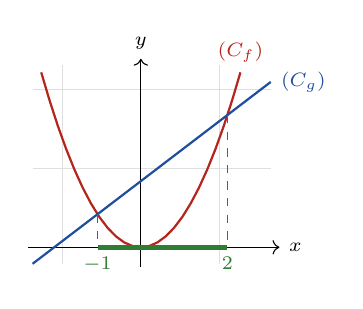
\begin{tikzpicture}[x=0.55cm,y=0.42cm,font=\scriptsize]
\draw[gray!25] (-2.5,-0.5) grid (3,5.5);
\draw[->] (-2.6,0)--(3.2,0) node[right]{$x$}; \draw[->] (0,-0.6)--(0,5.7) node[above]{$y$};
\draw[cThm,thick,domain=-2.3:2.3] plot (\x,{\x*\x}) node[above]{$(C_f)$};
\draw[cDef,thick] (-2.5,-0.5)--(3,5) node[right]{$(C_g)$};
\draw[cRem,dashed] (-1,1)--(-1,0) node[below]{$-1$} (2,4)--(2,0) node[below]{$2$};
\draw[cRem,line width=1.6pt] (-1,0)--(2,0);
\end{tikzpicture}\end{LTR}\par}{}{}
\Row{}{%
\Lab{cThm!80!black}{حذار}\ القراءة البيانية تقريبية ؛ نتحقق جبرياً عند الإمكان.}{}{}
\Row{التقويم}{%
\Lab{cEx}{تطبيق}\par $f(x)=x^2-2x$. \Num{1} بالحاسبة البيانية ارسم $(C_f)$. \Num{2} حل بيانياً $f(x)=0$ و $f(x)<0$. \Num{3} تحقق جبرياً.\par\textbf{الحل:} \Num{2} $\{0;2\}$ و $]0;2[$ ؛ \Num{3} $x^2-2x=x(x-2)$.\par\textbf{واجب منزلي:} تمارين من الكتاب المدرسي.\par\smallskip\textbf{ملاحظات حول سير الحصة:} \dotfill}{25 د}{باستعمال الحاسبة البيانية.}
\end{Sayr}
\newpage
\ModhHead{14}{1 ج م ع ت}{تحليل}{عموميات على الدوال}{02 سا}{اتجاه تغير دالة وجدول التغيرات}%
{\begin{itemize}\item التمثيل البياني لدالة.\item خواص الترتيب.\end{itemize}}%
{\begin{itemize}\item تعريف اتجاه تغير دالة.\item الانتقال من جدول التغيرات إلى التمثيل البياني والعكس.\end{itemize}}%
{المنهاج ، الكتاب المدرسي ، مراجع ، الحاسبة البيانية.}
\begin{Sayr}
\Row{مرحلة الانطلاق}{%
\textbf{التهيئة النفسية:} منحنى درجة الحرارة خلال يوم: متى ترتفع؟ متى تنخفض؟}{10 د}{حوار حول ظاهرة مألوفة.}
\Row{التشخيص والاكتشاف}{%
\Lab{cEx}{مناقشة نشاط 05 صفحة 50}\par\ck\ التحويل من الدرجة المئوية إلى فهرنهايت دالة تآلفية: $F=1{,}8\,C+32$ ، والنقطتان $A(0;32)$ و $B(100;212)$ من تمثيلها.\par
\ck\ كلما زادت $C$ زادت $F$: الدالة \textbf{متزايدة}.\par
\ck\ معامل التوجيه $\dfrac{212-32}{100}=1{,}8>0$.\par
}{35 د}{عمل ثنائي.}
\Row{بناء المعارف}{%
\Lab{cDef}{تعريف}\ $f$ دالة و $I$ مجال من $D_f$:\par\ck\ $f$ \textbf{متزايدة تماماً} على $I$ إذا كان من أجل كل $a<b$ من $I$: $f(a)<f(b)$.\par
\ck\ $f$ \textbf{متناقصة تماماً} على $I$ إذا كان من أجل كل $a<b$ من $I$: $f(a)>f(b)$.\par
\ck\ $f$ \textbf{ثابتة} على $I$ إذا كان $f(a)=f(b)$ لكل $a$ و $b$ من $I$.\par
\Lab{cThm}{جدول التغيرات}\ نلخص اتجاه التغير بأسهم: صاعد (متزايدة) ، نازل (متناقصة). مثلاً للدالة $f(x)=x^2$:\par\smallskip\begin{LTR}\centering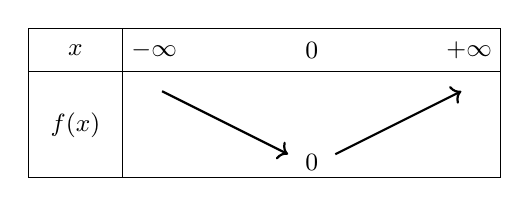
\begin{tikzpicture}[font=\small]
\draw (0,0) rectangle (6,1.9); \draw (0,1.35)--(6,1.35); \draw (1.2,0)--(1.2,1.9);
\node at (0.6,1.62){$x$}; \node at (0.6,0.67){$f(x)$};
\node at (1.6,1.62){$-\infty$}; \node at (3.6,1.62){$0$}; \node at (5.6,1.62){$+\infty$};
\node at (3.6,0.2){$0$};
\draw[->,thick] (1.7,1.1)--(3.3,0.3); \draw[->,thick] (3.9,0.3)--(5.5,1.1);
\end{tikzpicture}\end{LTR}\par}{50 د}{نرسم جدول التغيرات ونقابله بالمنحنى.}
\Row{}{%
\Lab{cEx}{مثال}\par\ck\ $f(x)=-3x+2$: إذا كان $a<b$ فإن $-3a>-3b$ ومنه $f(a)>f(b)$: متناقصة تماماً على $\R$.\par
\ck\ $g(x)=x^2$ على $[0;+\infty[$: إذا كان $0\leqslant a<b$ فإن $a^2<b^2$: متزايدة تماماً.\par
\Lab{cThm!80!black}{حذار}\ لا علاقة بين اتجاه التغير والإشارة: دالة سالبة قد تكون متزايدة.}{}{}
\Row{التقويم}{%
\Lab{cEx}{تطبيق}\par\Num{1} ادرس اتجاه تغير $h(x)=2x-5$ على $\R$. \Num{2} ارسم منحنياً ممكناً لدالة $f$ معرفة على $[-3;4]$ متزايدة على $[-3;1]$ ومتناقصة على $[1;4]$ مع $f(-3)=-1$ ، $f(1)=3$ ، $f(4)=0$.\par\textbf{الحل:} \Num{1} $a<b\Rightarrow2a-5<2b-5$: متزايدة تماماً.\par\textbf{واجب منزلي:} تمارين من الكتاب المدرسي.\par\smallskip\textbf{ملاحظات حول سير الحصة:} \dotfill}{25 د}{لكل تلميذ منحنى مختلف: نقارن.}
\end{Sayr}
\newpage
\ModhHead{15}{1 ج م ع ت}{تحليل}{عموميات على الدوال}{02 سا}{القيم الحدية لدالة}%
{\begin{itemize}\item اتجاه التغير وجدول التغيرات.\item المتطابقات الشهيرة.\end{itemize}}%
{\begin{itemize}\item تعريف القيمة الحدية العظمى والصغرى.\item تعيين القيم الحدية بالحاسبة البيانية وبالحساب.\end{itemize}}%
{المنهاج ، الكتاب المدرسي ، مراجع ، الحاسبة البيانية.}
\begin{Sayr}
\Row{مرحلة الانطلاق}{%
\textbf{التهيئة النفسية:} قذيفة ترتفع ثم تنزل: ما أعلى ارتفاع تبلغه؟}{10 د}{ربط بالواقع.}
\Row{التشخيص والاكتشاف}{%
\Lab{cEx}{وضعية مقترحة}\par مستطيل محيطه $20$ cm وأحد بعديه $x$. \Num{1} عبّر عن مساحته $A(x)$. \Num{2} بالحاسبة: ما قيمة $x$ التي تجعل المساحة أكبر ما يمكن؟\par\ck\ البعد الآخر $10-x$ ، و $A(x)=x(10-x)$ حيث $x\in]0;10[$.\par
\ck\ الجدول: $A(4)=24$ ، $A(5)=25$ ، $A(6)=24$: \textbf{تخمين} أعظم مساحة $25$ عند $x=5$ (مربع).\par
\ck\ \textbf{إثبات:} $A(x)=25-(x-5)^2\leqslant25$ و $A(5)=25$.\par
}{35 د}{عمل بالحاسبة البيانية في مجموعات.}
\Row{بناء المعارف}{%
\Lab{cDef}{تعريف}\ $f$ دالة معرفة على مجال $I$ و $a\in I$:\par\ck\ $f(a)$ \textbf{قيمة حدية عظمى} لـ $f$ على $I$ إذا كان $f(x)\leqslant f(a)$ لكل $x\in I$.\par
\ck\ $f(a)$ \textbf{قيمة حدية صغرى} إذا كان $f(x)\geqslant f(a)$ لكل $x\in I$.\par
\Lab{cMeth}{إثبات قيمة حدية}\ نكتب $f(x)$ على شكل $m+(\ldots)^2$ (صغرى) أو $M-(\ldots)^2$ (عظمى) ، ونعيّن القيمة التي تبلغها.\par}{50 د}{نؤكد الفرق بين التخمين والبرهان.}
\Row{}{%
\Lab{cEx}{مثال}\ $f(x)=x^2-4x+5=(x-2)^2+1\geqslant1$ و $f(2)=1$: القيمة الحدية الصغرى $1$ عند $x=2$.\par\Lab{cRem}{ملاحظات}\ نقرأ القيم الحدية من جدول التغيرات: عند تغيّر اتجاه السهم.\par}{}{}
\Row{}{%
\Lab{cThm!80!black}{حذار}\ الحاسبة تعطي \textbf{تخميناً} لا برهاناً.}{}{}
\Row{التقويم}{%
\Lab{cEx}{تطبيق}\par عيّن القيمة الحدية لكل دالة: \Num{1} $g(x)=-x^2+2x+3$ ؛ \Num{2} $h(x)=x^2+6x+10$.\par\textbf{الحل:} \Num{1} $g(x)=4-(x-1)^2$: عظمى $4$ عند $1$ ؛ \Num{2} $h(x)=(x+3)^2+1$: صغرى $1$ عند $-3$.\par\textbf{واجب منزلي:} تمارين من الكتاب المدرسي.\par\smallskip\textbf{ملاحظات حول سير الحصة:} \dotfill}{25 د}{تقويم فردي.}
\end{Sayr}
\newpage
\ModhHead{16}{1 ج م ع ت}{تحليل}{عموميات على الدوال}{02 سا}{شفعية دالة والبرهان بمثال مضاد}%
{\begin{itemize}\item التناظر المحوري والمركزي.\item مجموعة تعريف دالة.\end{itemize}}%
{\begin{itemize}\item التعرّف على دالة زوجية أو فردية.\item التفسير البياني للشفعية.\item البرهان بمثال مضاد.\end{itemize}}%
{المنهاج ، الكتاب المدرسي ، مراجع ، الحاسبة البيانية.}
\begin{Sayr}
\Row{مرحلة الانطلاق}{%
\textbf{التهيئة النفسية:} صورة فراشة: ما الذي تلاحظه؟ ارسم نظير نقطة بالنسبة إلى محور التراتيب.}{10 د}{صورة من الطبيعة.}
\Row{التشخيص والاكتشاف}{%
\Lab{cEx}{مناقشة نشاط 04 صفحة 50}\par\ck\ $f(x)=x^4-2x^2$ على $[-2;2]$: $f(2)=f(-2)=8$ و $f(1)=f(-1)=-1$.\par
\ck\ من أجل كل $x$ من $[-2;2]$: $-x\in[-2;2]$ و $f(-x)=(-x)^4-2(-x)^2=f(x)$.\par
\ck\ النقطتان $M(x;f(x))$ و $M_1(-x;f(x))$ متناظرتان بالنسبة إلى محور التراتيب: المنحنى متناظر.\par
}{35 د}{عمل ثنائي على التمثيل البياني.}
\Row{بناء المعارف}{%
\Lab{cDef}{تعريف}\ $D_f$ متناظرة بالنسبة إلى $0$:\par\ck\ $f$ \textbf{زوجية} إذا كان $f(-x)=f(x)$ لكل $x\in D_f$.\par
\ck\ $f$ \textbf{فردية} إذا كان $f(-x)=-f(x)$ لكل $x\in D_f$.\par
\Lab{cThm}{التفسير البياني}\ $f$ زوجية $\iff$ $(C_f)$ متناظر بالنسبة إلى محور التراتيب ؛ $f$ فردية $\iff$ $(C_f)$ متناظر بالنسبة إلى المبدأ $O$.\par}{50 د}{نرسم المنحنيين النموذجيين على السبورة.}
\Row{}{%
\Lab{cEx}{مثال}\par\ck\ $x\mapsto x^2+1$ زوجية ؛ $x\mapsto x^3-x$ فردية.\par
\ck\ $k(x)=\dfrac{1}{x-1}$: $D_k=\R-\{1\}$ غير متناظرة ، إذن $k$ ليست زوجية ولا فردية.\par
\Lab{cMeth}{البرهان بمثال مضاد}\ لإثبات أن خاصية «من أجل كل $x$» خاطئة يكفي مثال واحد: $h(x)=x^2+x$ ليست زوجية لأن $h(-1)=0\ne h(1)=2$ ، وليست فردية لأن $h(-1)\ne-h(1)$.\par}{}{}
\Row{}{%
\Lab{cThm!80!black}{حذار}\ الأمثلة لا تكفي لإثبات أن خاصية صحيحة.}{}{}
\Row{التقويم}{%
\Lab{cEx}{تطبيق}\par ادرس شفعية: \Num{1} $f(x)=\dfrac{x}{x^2+1}$ ؛ \Num{2} $g(x)=|x|+x^2$ ؛ \Num{3} $k(x)=2x+1$.\par\textbf{الحل:} \Num{1} $f(-x)=-f(x)$: فردية ؛ \Num{2} $g(-x)=g(x)$: زوجية ؛ \Num{3} $k(1)=3$ و $k(-1)=-1$: ليست زوجية ولا فردية.\par\textbf{واجب منزلي:} تمارين حوصلة المحور من الكتاب المدرسي.\par\smallskip\textbf{ملاحظات حول سير الحصة:} \dotfill}{25 د}{نهاية المحور: فرض أو تمارين حوصلة.}
\end{Sayr}
\end{document}
